\documentclass[aspectratio=169,10pt]{beamer}

% ─── Tema ────────────────────────────────────────────────────────────────────
\usetheme{Madrid}
\usecolortheme{seahorse}
\usefonttheme{professionalfonts}
\setbeamertemplate{navigation symbols}{}
\setbeamertemplate{footline}[frame number]
\setbeamertemplate{itemize items}[circle]

% ─── Paquetes ─────────────────────────────────────────────────────────────────
\usepackage[utf8]{inputenc}
\usepackage[T1]{fontenc}
\usepackage[english]{babel}  % spanish.ldf no disponible; contenido en español igual
\usepackage{amsmath, amssymb}
\usepackage{graphicx}
\usepackage{booktabs}
\usepackage{xcolor}
\usepackage{listings}
\usepackage{tikz}
\usetikzlibrary{shapes.geometric, arrows.meta, positioning, fit, backgrounds}
\usepackage{pifont}
\usepackage{hyperref}
\usepackage{tcolorbox}
\tcbuselibrary{listingsutf8, skins}

% ─── Colores ──────────────────────────────────────────────────────────────────
\definecolor{pyblue}{HTML}{306998}
\definecolor{pyorange}{HTML}{FFD43B}
\definecolor{lightgray}{HTML}{F5F5F5}
\definecolor{darkgreen}{HTML}{1B5E20}
\definecolor{codegreen}{RGB}{40,180,99}
\definecolor{codepurple}{RGB}{142,68,173}
\definecolor{codegray}{RGB}{127,140,141}
\definecolor{backcolour}{RGB}{250,250,250}

% ─── Estilo de código ─────────────────────────────────────────────────────────
\lstdefinestyle{pythonstyle}{
    backgroundcolor=\color{backcolour},
    commentstyle=\color{codegray}\itshape,
    keywordstyle=\color{pyblue}\bfseries,
    stringstyle=\color{codegreen},
    basicstyle=\ttfamily\scriptsize,
    breaklines=true,
    captionpos=b,
    keepspaces=true,
    showspaces=false,
    showstringspaces=false,
    tabsize=2,
    frame=single,
    rulecolor=\color{pyblue!40},
    language=Python,
    morekeywords={self, True, False, None, def, class, return, import, from, as},
}

\lstdefinestyle{yamlstyle}{
    backgroundcolor=\color{backcolour},
    basicstyle=\ttfamily\scriptsize,
    keywordstyle=\color{pyblue}\bfseries,
    stringstyle=\color{codegreen},
    commentstyle=\color{codegray}\itshape,
    breaklines=true,
    frame=single,
    rulecolor=\color{pyblue!40},
}

\lstdefinestyle{bashstyle}{
    backgroundcolor=\color{black!90},
    basicstyle=\ttfamily\scriptsize\color{white},
    breaklines=true,
    frame=single,
    rulecolor=\color{black},
}

% ─── Sustitutos de fontawesome (sin paquete externo) ─────────────────────────
\newcommand{\faIcon}[1]{\textbullet}
\newcommand{\faChalkboardTeacher}{\ding{45}}
\newcommand{\faLightbulb}{\ding{171}}

% ─── Bloque de nota para el maestro ──────────────────────────────────────────
\newcommand{\teachernote}[1]{%
    \begin{tcolorbox}[
        colback=pyorange!20, colframe=pyorange!80!black,
        fonttitle=\bfseries\small, title={\faLightbulb\ Nota docente},
        left=4pt, right=4pt, top=2pt, bottom=2pt, sharp corners
    ]
    \scriptsize #1
    \end{tcolorbox}
}

% ─── Comando de archivo ───────────────────────────────────────────────────────
\newcommand{\codefile}[1]{\texttt{\textcolor{pyblue}{#1}}}

% ─── Metadatos ────────────────────────────────────────────────────────────────
\title[Clasificación con PyTorch Lightning]{%
    \textbf{Clasificación de Imágenes con PyTorch Lightning}\\
    \large Perros vs.\ Gatos --- Proyecto de Clase}
\subtitle{Arquitecturas de Sistemas de Inteligencia Artificial}
\author[CUGDL]{\faChalkboardTeacher\quad Clase de Arquitecturas de Redes Neuronales\\[4pt]
    \small \texttt{CUGDL --- Comunidad Universitaria de Guadalajara en Deep Learning}}
\date{\today}
\titlegraphic{\vspace{-8pt}}

%==============================================================================
\begin{document}
%==============================================================================

% ── Portada ──────────────────────────────────────────────────────────────────
\begin{frame}[plain]
    \titlepage
\end{frame}

% ── Índice ───────────────────────────────────────────────────────────────────
\begin{frame}{Contenido}
    \tableofcontents
\end{frame}

%==============================================================================
\section{Motivación y Objetivos}
%==============================================================================

\begin{frame}{¿Por qué este proyecto?}
    \begin{columns}
        \column{0.55\textwidth}
        \textbf{Objetivos de aprendizaje:}
        \begin{itemize}
            \item Comprender el \textbf{flujo completo} de un proyecto de visión artificial
            \item Aprender el patrón \textbf{LightningModule} para organizar código de entrenamiento
            \item Practicar \textbf{data augmentation} y normalización de imágenes
            \item Separar correctamente \textbf{train / val / test}
            \item Usar \textbf{TensorBoard} para monitorear experimentos
            \item Gestionar hiperparámetros con \textbf{archivos YAML}
        \end{itemize}

        \column{0.42\textwidth}
        \begin{tcolorbox}[colback=pyblue!10, colframe=pyblue, title=Stack tecnológico]
            \small
            \faIcon{python}\ \textbf{Python 3.10}\\[4pt]
            \faIcon{fire}\ \textbf{PyTorch 2.7} + CUDA 12.6\\[4pt]
            \faIcon{bolt}\ \textbf{PyTorch Lightning 2.6}\\[4pt]
            \faIcon{chart-line}\ \textbf{TensorBoard}\\[4pt]
            \faIcon{sliders}\ \textbf{LightningCLI + YAML}
        \end{tcolorbox}
    \end{columns}
\end{frame}

\begin{frame}{Problema: Clasificación Binaria de Imágenes}
    \begin{columns}
        \column{0.6\textwidth}
        \textbf{Tarea:} dado el tensor de una imagen RGB,\\
        predecir si contiene un \textbf{perro} o un \textbf{gato}.

        \vspace{8pt}
        Formalmente:
        \[
            f_\theta : \mathbb{R}^{3 \times H \times W} \;\longrightarrow\; \{0,\, 1\}
        \]
        donde $\theta$ son los parámetros aprendidos por la red.

        \vspace{8pt}
        \textbf{Función de pérdida:} Cross-Entropy
        \[
            \mathcal{L} = -\sum_{c=0}^{1} y_c \log \hat{p}_c
        \]

        \vspace{4pt}
        \textbf{Métrica principal:} Accuracy
        \[
            \text{Acc} = \frac{\text{predicciones correctas}}{\text{total de muestras}}
        \]

        \column{0.37\textwidth}
        \begin{tcolorbox}[colback=lightgray, colframe=gray!50]
            \centering
            \small
            \textbf{Clases}\\[6pt]
            \begin{tabular}{cl}
                \toprule
                Índice & Clase \\
                \midrule
                0 & \faIcon{dog}\ perro \\
                1 & \faIcon{cat}\ gato  \\
                \bottomrule
            \end{tabular}\\[8pt]
            \small $\approx 194$ imágenes totales\\
            descargadas con la API\\
            \texttt{dog.ceo} y Cataas
        \end{tcolorbox}
    \end{columns}
\end{frame}

%==============================================================================
\section{Estructura del Proyecto}
%==============================================================================

\begin{frame}{Organización del Repositorio}
    \begin{columns}
        \column{0.48\textwidth}
        \begin{tcolorbox}[colback=lightgray, colframe=pyblue!60, title=Archivos principales]
        \scriptsize
        \begin{tabular}{ll}
            \codefile{main.py}     & Punto de entrada (CLI)    \\
            \codefile{model.py}    & Arquitecturas + LightningModule \\
            \codefile{dataset.py}  & Dataset + DataModule      \\
            \codefile{utils.py}    & Semillas y auxiliares     \\
            \codefile{config.py}   & Constantes (legado)       \\
        \end{tabular}
        \end{tcolorbox}

        \vspace{4pt}
        \begin{tcolorbox}[colback=lightgray, colframe=pyorange!80, title=Configuración]
        \scriptsize
        \begin{tabular}{ll}
            \codefile{configs/fit.yaml} & Entrenamiento    \\
            \codefile{configs/val.yaml} & Validación/Test  \\
        \end{tabular}
        \end{tcolorbox}

        \column{0.48\textwidth}
        \begin{tcolorbox}[colback=lightgray, colframe=codegreen!80, title=Datos y artefactos]
        \scriptsize
        \begin{tabular}{ll}
            \codefile{data/dogs/}  & Imágenes de perros      \\
            \codefile{data/cats/}  & Imágenes de gatos       \\
            \codefile{models/}     & Checkpoints (.ckpt)     \\
            \codefile{runs/dogcat/} & Logs de TensorBoard    \\
            \quad\codefile{version\_0/} &                    \\
            \quad\codefile{version\_1/} &                    \\
        \end{tabular}
        \end{tcolorbox}
    \end{columns}

    \vspace{6pt}
    \teachernote{Destacar que \texttt{configs/} separa \emph{qué} hace el código de \emph{cómo} está configurado. Esto facilita reproducibilidad y experimentación.}
\end{frame}

%==============================================================================
\section{Pipeline de Datos}
%==============================================================================

\begin{frame}{Dataset y División Train / Val / Test}
    \begin{columns}
        \column{0.52\textwidth}

        \textbf{Clase \texttt{DogCatDataset}:}\\
        \begin{itemize}
            \item Lee imágenes de \codefile{data/dogs/} y \codefile{data/cats/}
            \item Devuelve tupla \texttt{(tensor, label)}
            \item Soporta transform personalizado por split
        \end{itemize}

        \vspace{8pt}
        \textbf{Clase \texttt{DogCatDataModule}:}\\
        \begin{itemize}
            \item Hereda de \texttt{L.LightningDataModule}
            \item Método \texttt{setup()} divide el dataset con semilla fija
            \item Expone \texttt{train/val/test\_dataloader()}
        \end{itemize}

        \column{0.45\textwidth}

        \begin{center}
        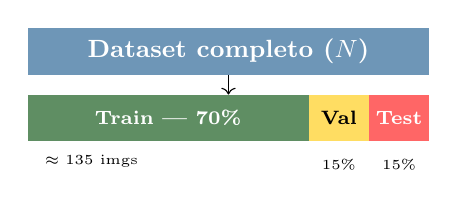
\begin{tikzpicture}[scale=0.85]
            % barra total
            \fill[pyblue!70]   (0,0) rectangle (6.0, 0.7) node[midway, white, font=\small\bfseries] {Dataset completo ($N$)};

            % splits
            \fill[darkgreen!70]  (0,-1.0) rectangle (4.2, -0.3) node[midway, white, font=\scriptsize\bfseries] {Train --- 70\%};
            \fill[pyorange!80]   (4.2,-1.0) rectangle (5.1, -0.3) node[midway, black, font=\scriptsize\bfseries] {Val};
            \fill[red!60]        (5.1,-1.0) rectangle (6.0, -0.3) node[midway, white, font=\scriptsize\bfseries] {Test};

            \draw[->] (3.0, -0.0) -- (3.0, -0.3);
            \node[font=\tiny] at (0.95, -1.3)  {$\approx 135$ imgs};
            \node[font=\tiny] at (4.65, -1.35) {15\%};
            \node[font=\tiny] at (5.55, -1.35) {15\%};
        \end{tikzpicture}
        \end{center}

        \vspace{6pt}
        \begin{tcolorbox}[colback=lightgray, colframe=gray!50]
            \scriptsize
            \texttt{random\_split} con \texttt{Generator(seed=42)}\\
            $\Rightarrow$ partición \textbf{reproducible}
        \end{tcolorbox}
    \end{columns}
\end{frame}

\begin{frame}[fragile]{Data Augmentation por Split}

    \begin{columns}
        \column{0.52\textwidth}
        \begin{lstlisting}[style=pythonstyle, title=build\_transforms()]
def build_transforms(img_size, mean, std,
                     augment=False):
    steps = [Resize((img_size, img_size))]

    if augment:           # solo en TRAIN
        steps += [
            RandomHorizontalFlip(p=0.5),
            RandomRotation(10),
        ]

    steps += [
        ToTensor(),
        Normalize(mean, std),  # ImageNet stats
    ]
    return Compose(steps)
        \end{lstlisting}

        \column{0.44\textwidth}

        \begin{tcolorbox}[colback=lightgray, colframe=pyblue!60, title=\scriptsize Transforms por split]
            \scriptsize
            \begin{tabular}{lcc}
                \toprule
                Transform & Train & Val/Test \\
                \midrule
                Resize $224\times224$ & \checkmark & \checkmark \\
                H-Flip ($p=0.5$)      & \checkmark & \texttimes \\
                Rotation ($\pm10°$)   & \checkmark & \texttimes \\
                ToTensor              & \checkmark & \checkmark \\
                Normalize (ImageNet)  & \checkmark & \checkmark \\
                \bottomrule
            \end{tabular}
        \end{tcolorbox}

        \vspace{4pt}
        \teachernote{Preguntar: ¿Por qué NO aplicamos augmentation en val/test? La respuesta guía la discusión de \emph{data leakage}.}
    \end{columns}
\end{frame}

%==============================================================================
\section{Arquitecturas de Red}
%==============================================================================

\begin{frame}{SimpleCNN --- Arquitectura Propia}

    \begin{center}
    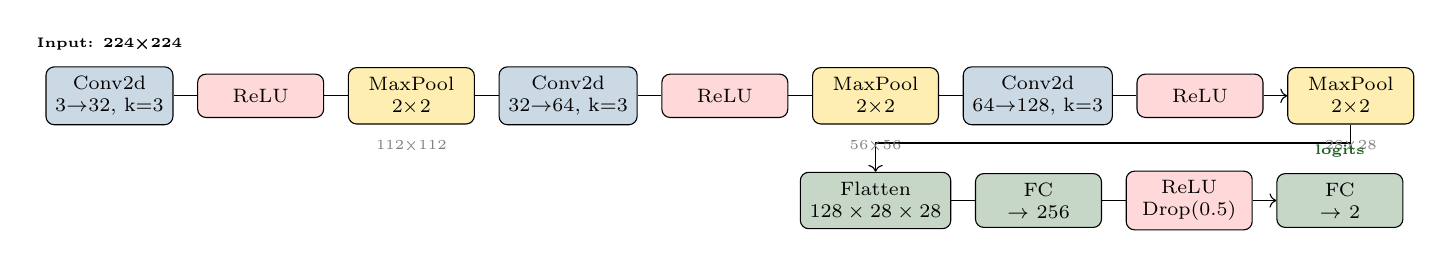
\begin{tikzpicture}[
        node distance=0.45cm and 0.3cm,
        box/.style={draw, rounded corners=3pt, minimum width=1.6cm,
                    minimum height=0.55cm, font=\scriptsize, align=center},
        conv/.style={box, fill=pyblue!25},
        pool/.style={box, fill=pyorange!40},
        fc/.style={box, fill=darkgreen!25},
        op/.style={box, fill=red!15},
    ]
        \node[conv] (c1) {Conv2d\\3$\to$32, k=3};
        \node[op,   right=of c1] (r1) {ReLU};
        \node[pool, right=of r1] (p1) {MaxPool\\2×2};

        \node[conv, right=of p1] (c2) {Conv2d\\32$\to$64, k=3};
        \node[op,   right=of c2] (r2) {ReLU};
        \node[pool, right=of r2] (p2) {MaxPool\\2×2};

        \node[conv, right=of p2] (c3) {Conv2d\\64$\to$128, k=3};
        \node[op,   right=of c3] (r3) {ReLU};
        \node[pool, right=of r3] (p3) {MaxPool\\2×2};

        \draw[->] (c1)--(r1)--(p1)--(c2)--(r2)--(p2)--(c3)--(r3)--(p3);

        % Flatten + FC
        \node[fc,  below=0.6cm of p2] (flat) {Flatten\\$128\times28\times28$};
        \node[fc,  right=of flat] (fc1) {FC\\$\to$ 256};
        \node[op,  right=of fc1]  (r4)  {ReLU\\Drop(0.5)};
        \node[fc,  right=of r4]   (fc2) {FC\\$\to$ 2};

        \draw[->] (p3) -- ++(0,-0.6cm) -| (flat);
        \draw[->] (flat)--(fc1)--(r4)--(fc2);

        % Anotaciones de tamaño
        \node[below=0.08cm of p1, font=\tiny, gray] {112×112};
        \node[below=0.08cm of p2, font=\tiny, gray] {56×56};
        \node[below=0.08cm of p3, font=\tiny, gray] {28×28};
        \node[above=0.08cm of c1, font=\tiny\bfseries] {Input: 224×224};
        \node[above=0.08cm of fc2, font=\tiny\bfseries, darkgreen] {logits};
    \end{tikzpicture}
    \end{center}

    \vspace{4pt}
    \begin{columns}
        \column{0.5\textwidth}
        \begin{tcolorbox}[colback=lightgray, colframe=pyblue!50]
            \scriptsize
            \textbf{Parámetros totales:} 25.8 M\\
            Capa más costosa: \texttt{FC 128·28·28 $\to$ 256}\\
            $= 128 \times 784 \times 256 + 256 \approx 25.7\text{M}$
        \end{tcolorbox}

        \column{0.46\textwidth}
        \teachernote{Discutir el crecimiento cuadrático de parámetros en la capa FC y por qué GlobalAveragePooling lo soluciona (ResNet-style).}
    \end{columns}
\end{frame}

\begin{frame}[fragile]{ResNet-18 --- Transfer Learning}
    \begin{columns}
        \column{0.52\textwidth}
        \textbf{¿Qué es Transfer Learning?}
        \begin{itemize}
            \item Red preentrenada en \textbf{ImageNet} (1.2 M imágenes, 1000 clases)
            \item Los primeros bloques extraen características generales:\\
                  bordes, texturas, formas
            \item \textbf{Solo reemplazamos} la capa final
        \end{itemize}

        \vspace{6pt}
        \begin{lstlisting}[style=pythonstyle]
net = resnet18(weights=ResNet18_Weights.DEFAULT)
# Reemplazar cabeza clasificadora
net.fc = nn.Linear(net.fc.in_features, num_classes)
        \end{lstlisting}

        \column{0.44\textwidth}
        \begin{tcolorbox}[colback=lightgray, colframe=pyblue!60]
            \scriptsize\centering
            \begin{tabular}{lcc}
                \toprule
                & SimpleCNN & ResNet-18 \\
                \midrule
                Parámetros  & 25.8 M & 11.2 M \\
                Preentrenado & No     & Sí (ImageNet) \\
                Conv. bloques & 3     & 8 residuales \\
                Global Pool  & No    & Sí (GAP) \\
                \bottomrule
            \end{tabular}
        \end{tcolorbox}

        \vspace{4pt}
        Selección desde YAML:
        \begin{lstlisting}[style=yamlstyle]
model:
  backbone: resnet18   # o simplecnn
  pretrained: true
        \end{lstlisting}
    \end{columns}
\end{frame}

%==============================================================================
\section{PyTorch Lightning}
%==============================================================================

\begin{frame}{¿Por qué PyTorch Lightning?}
    \begin{columns}
        \column{0.5\textwidth}
        \textbf{Problema con PyTorch vanilla:}
        \begin{itemize}
            \item El loop de entrenamiento es \textbf{código boilerplate}
            \item Gestión manual de \texttt{.train()}, \texttt{.eval()}, \texttt{.to(device)}
            \item Acumulación de gradientes, logging\ldots\ todo manual
            \item Difícil escalar a multi-GPU o TPU
        \end{itemize}

        \column{0.46\textwidth}
        \textbf{Lightning separa responsabilidades:}
        \begin{tcolorbox}[colback=lightgray, colframe=pyblue!60]
            \scriptsize
            \begin{tabular}{ll}
                \toprule
                Clase & Responsabilidad \\
                \midrule
                \texttt{LightningModule}  & Modelo + pasos \\
                \texttt{LightningDataModule} & Datos \\
                \texttt{Trainer}          & Loop + hardware \\
                \texttt{LightningCLI}     & Config YAML/CLI \\
                \bottomrule
            \end{tabular}
        \end{tcolorbox}
    \end{columns}

    \vspace{8pt}
    \begin{center}
    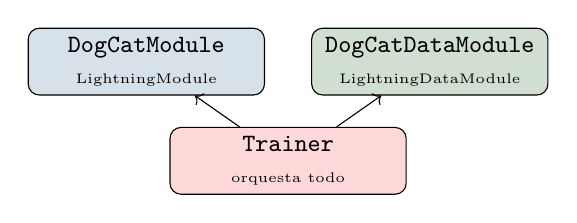
\begin{tikzpicture}[scale=0.9,
        box/.style={draw, rounded corners=4pt, minimum width=3cm,
                    minimum height=0.7cm, font=\small, align=center, fill=#1}
    ]
        \node[box=pyblue!20]  (lm)   at (0,0)    {\texttt{DogCatModule}\\{\tiny LightningModule}};
        \node[box=darkgreen!20] (dm) at (4,0)    {\texttt{DogCatDataModule}\\{\tiny LightningDataModule}};
        \node[box=red!15]     (tr)   at (2,-1.4) {\texttt{Trainer}\\{\tiny orquesta todo}};
        \draw[->] (tr) -- (lm);
        \draw[->] (tr) -- (dm);
    \end{tikzpicture}
    \end{center}
\end{frame}

\begin{frame}[fragile]{\texttt{DogCatModule} --- LightningModule}
    \begin{lstlisting}[style=pythonstyle]
class DogCatModule(L.LightningModule):
    def __init__(self, num_classes=2, lr=1e-3, momentum=0.9,
                 backbone="simplecnn", pretrained=True):
        super().__init__()
        self.save_hyperparameters()   # guarda todos los args en hparams
        self.net = SimpleCNN(num_classes) if backbone=="simplecnn" \
                   else _build_resnet18(num_classes, pretrained)
        self.criterion  = nn.CrossEntropyLoss()
        self.train_acc  = torchmetrics.Accuracy(task="multiclass", num_classes=2)
        self.val_acc    = torchmetrics.Accuracy(task="multiclass", num_classes=2)

    def training_step(self, batch, batch_idx):
        x, y = batch
        logits = self(x)
        loss   = self.criterion(logits, y)
        self.log("train/loss", loss, on_epoch=True, prog_bar=True)
        return loss

    def configure_optimizers(self):
        return torch.optim.SGD(self.parameters(),
                               lr=self.hparams.lr,
                               momentum=self.hparams.momentum)
    \end{lstlisting}

    \vspace{-4pt}
    \teachernote{Señalar \texttt{save\_hyperparameters()} --- guarda automáticamente los hiperparámetros en el checkpoint y en TensorBoard. Discutir por qué \texttt{training\_step} solo retorna la pérdida.}
\end{frame}

\begin{frame}[fragile]{LightningCLI --- Configuración por YAML}

    \begin{columns}
        \column{0.48\textwidth}
        \begin{lstlisting}[style=pythonstyle, title=main.py (punto de entrada)]
from lightning.pytorch.cli import LightningCLI
from model   import DogCatModule
from dataset import DogCatDataModule

def main():
    torch.set_float32_matmul_precision("high")
    LightningCLI(DogCatModule, DogCatDataModule)
        \end{lstlisting}

        \vspace{6pt}
        \begin{lstlisting}[style=bashstyle]
# Entrenar
python main.py fit \
    --config configs/fit.yaml

# Sobreescribir un param
python main.py fit \
    --config configs/fit.yaml \
    --trainer.max_epochs 20
        \end{lstlisting}

        \column{0.48\textwidth}
        \begin{lstlisting}[style=yamlstyle, title=configs/fit.yaml (fragmento)]
seed_everything: 42

trainer:
  max_epochs: 10
  accelerator: auto
  logger:
    class_path: ...TensorBoardLogger
    init_args:
      save_dir: runs
      name: dogcat

model:
  backbone: simplecnn
  lr: 0.001

data:
  batch_size: 32
  train_ratio: 0.70
  val_ratio:   0.15
        \end{lstlisting}
    \end{columns}
\end{frame}

%==============================================================================
\section{Callbacks y Monitoreo}
%==============================================================================

\begin{frame}{Callbacks Activos}

    \begin{columns}
        \column{0.32\textwidth}
        \begin{tcolorbox}[colback=darkgreen!10, colframe=darkgreen!70,
                          title={\scriptsize\faIcon{save}\ ModelCheckpoint}]
            \scriptsize
            \begin{itemize}
                \item Monitorea \texttt{val/acc}
                \item Guarda el \textbf{mejor} modelo
                \item Archivo: \codefile{models/best\_model.ckpt}
            \end{itemize}
        \end{tcolorbox}

        \column{0.32\textwidth}
        \begin{tcolorbox}[colback=red!10, colframe=red!70,
                          title={\scriptsize\faIcon{stop-circle}\ EarlyStopping}]
            \scriptsize
            \begin{itemize}
                \item Monitorea \texttt{val/loss}
                \item Paciencia: \textbf{4 épocas}
                \item Evita sobreentrenamiento
            \end{itemize}
        \end{tcolorbox}

        \column{0.32\textwidth}
        \begin{tcolorbox}[colback=pyblue!10, colframe=pyblue!70,
                          title={\scriptsize\faIcon{chart-bar}\ LRMonitor}]
            \scriptsize
            \begin{itemize}
                \item Registra el \textit{learning rate}
                \item Útil con schedulers
                \item Visible en TensorBoard
            \end{itemize}
        \end{tcolorbox}
    \end{columns}

    \vspace{10pt}
    \textbf{Métricas registradas por época:}

    \vspace{4pt}
    \begin{center}
    \begin{tabular}{llll}
        \toprule
        Métrica & Split & Descripción & \texttt{prog\_bar} \\
        \midrule
        \texttt{train/loss} & Train & Cross-Entropy & \checkmark \\
        \texttt{train/acc}  & Train & Accuracy       & \checkmark \\
        \texttt{val/loss}   & Val   & Cross-Entropy & \checkmark \\
        \texttt{val/acc}    & Val   & Accuracy       & \checkmark \\
        \texttt{test/loss}  & Test  & Cross-Entropy & --- \\
        \texttt{test/acc}   & Test  & Accuracy       & --- \\
        \bottomrule
    \end{tabular}
    \end{center}
\end{frame}

\begin{frame}[fragile]{TensorBoard --- Versionado de Experimentos}

    \begin{columns}
        \column{0.52\textwidth}
        \textbf{Estructura de logs:}
        \begin{center}
        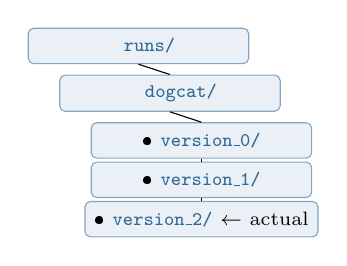
\begin{tikzpicture}[
            folder/.style={draw=pyblue!60, fill=pyblue!10, rounded corners=2pt,
                            minimum width=2.8cm, minimum height=0.45cm,
                            font=\scriptsize, align=left},
            every node/.style={font=\scriptsize},
        ]
            \node[folder] (runs)     at (0,0)    {\quad \codefile{runs/}};
            \node[folder] (dogcat)   at (0.4,-0.6) {\quad \codefile{dogcat/}};
            \node[folder] (v0)       at (0.8,-1.2) {\faIcon{check-circle}\ \codefile{version\_0/}};
            \node[folder] (v1)       at (0.8,-1.7) {\faIcon{check-circle}\ \codefile{version\_1/}};
            \node[folder] (v2)       at (0.8,-2.2) {\faIcon{clock}\ \codefile{version\_2/} $\leftarrow$ actual};
            \draw (runs.south) -- (dogcat.north);
            \draw (dogcat.south) -- (v0.north);
            \draw (v0.south) -- (v1.north);
            \draw (v1.south) -- (v2.north);
        \end{tikzpicture}
        \end{center}

        \column{0.44\textwidth}
        \begin{lstlisting}[style=bashstyle]
# Ver todos los experimentos
tensorboard --logdir runs

# Comparar dos versiones
tensorboard --logdir \
  v0:runs/dogcat/version_0,\
  v1:runs/dogcat/version_1
        \end{lstlisting}

        \vspace{6pt}
        \begin{tcolorbox}[colback=lightgray, colframe=pyorange!80]
            \scriptsize
            Cada \texttt{python main.py fit} crea \textbf{automáticamente} una nueva \texttt{version\_N} $\Rightarrow$ \textbf{ningún experimento se sobreescribe}
        \end{tcolorbox}
    \end{columns}
\end{frame}

%==============================================================================
\section{Flujo Completo y Resultados}
%==============================================================================

\begin{frame}{Flujo Completo del Proyecto}

    \begin{center}
    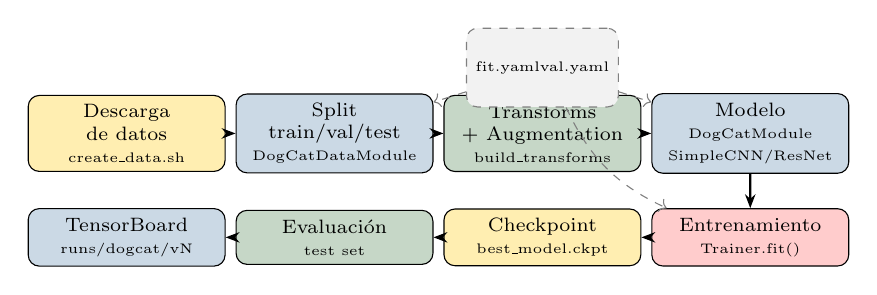
\begin{tikzpicture}[
        scale=0.88,
        step/.style={draw, rounded corners=4pt, minimum width=2.5cm,
                     minimum height=0.65cm, font=\scriptsize, align=center, fill=#1},
        arrow/.style={-{Stealth[length=5pt]}, thick},
    ]
        %--- Fila 1 ---
        \node[step=pyorange!40]   (data)  at (0,0)    {Descarga\\de datos\\{\tiny create\_data.sh}};
        \node[step=pyblue!25]     (split) at (3,0)    {Split\\train/val/test\\{\tiny DogCatDataModule}};
        \node[step=darkgreen!25]  (aug)   at (6,0)    {Transforms\\+ Augmentation\\{\tiny build\_transforms}};
        \node[step=pyblue!25]     (model) at (9,0)    {Modelo\\{\tiny DogCatModule}\\{\tiny SimpleCNN/ResNet}};

        \draw[arrow] (data)  -- (split);
        \draw[arrow] (split) -- (aug);
        \draw[arrow] (aug)   -- (model);

        %--- Fila 2 ---
        \node[step=red!20]        (train) at (9,-1.5) {Entrenamiento\\{\tiny Trainer.fit()}};
        \node[step=pyorange!40]   (ckpt)  at (6,-1.5) {Checkpoint\\{\tiny best\_model.ckpt}};
        \node[step=darkgreen!25]  (eval)  at (3,-1.5) {Evaluación\\{\tiny test set}};
        \node[step=pyblue!25]     (tb)    at (0,-1.5) {TensorBoard\\{\tiny runs/dogcat/vN}};

        \draw[arrow] (model) -- (train);
        \draw[arrow] (train) -- (ckpt);
        \draw[arrow] (ckpt)  -- (eval);
        \draw[arrow] (eval)  -- (tb);

        %--- YAML ---
        \node[draw=gray, dashed, rounded corners, font=\tiny,
              fill=gray!10, minimum width=1.8cm, minimum height=1.0cm]
              (yaml) at (6,0.95) {fit.yaml\\val.yaml};
        \draw[->, dashed, gray] (yaml) -- (split);
        \draw[->, dashed, gray] (yaml) -- (model);
        \draw[->, dashed, gray] (yaml) to[bend right=20] (train);
    \end{tikzpicture}
    \end{center}

    \vspace{4pt}
    \teachernote{Recorrer el diagrama con los alumnos y preguntar: ¿qué pasaría si entrenamos sin split de validación? ¿Y sin EarlyStopping?}
\end{frame}

\begin{frame}{Resultados --- Ejecución de Prueba}

    \begin{columns}
        \column{0.52\textwidth}
        \textbf{Configuración usada:}
        \begin{itemize}
            \item Backbone: \texttt{SimpleCNN}
            \item 10 épocas, batch 32, lr = 0.001
            \item GPU: NVIDIA RTX 3070 Laptop
            \item Dataset: $\approx 194$ imágenes
        \end{itemize}

        \vspace{6pt}
        \begin{tcolorbox}[colback=lightgray, colframe=pyblue!60]
            \scriptsize\centering
            \begin{tabular}{lccc}
                \toprule
                Split & N & Loss & Accuracy \\
                \midrule
                Train & 135 & 0.689 & 0.511 \\
                Val   & 29  & 0.693 & 0.517 \\
                \bottomrule
            \end{tabular}
        \end{tcolorbox}

        \column{0.44\textwidth}
        \begin{tcolorbox}[colback=pyorange!15, colframe=pyorange!80, title=\scriptsize¿Por qué $\approx 50\%$?]
            \scriptsize
            El dataset es muy pequeño ($\approx 100$ imgs/clase). La red aprende patrones estadísticos insuficientes.\\[6pt]
            \textbf{Soluciones a discutir:}
            \begin{enumerate}
                \item Usar \textbf{ResNet-18} preentrenada
                \item Aumentar el dataset ($>1000$ imgs)
                \item Aplicar más augmentation
                \item Ajustar learning rate / scheduler
            \end{enumerate}
        \end{tcolorbox}
    \end{columns}
\end{frame}

%==============================================================================
\section{Comandos y Ejercicios}
%==============================================================================

\begin{frame}[fragile]{Comandos Principales}

    \begin{columns}
        \column{0.48\textwidth}
        \begin{lstlisting}[style=bashstyle, title=Preparación]
# Activar entorno
conda activate pytorch

# Instalar dependencias
pip install -r requirements.txt

# Descargar dataset
bash create_data.sh
        \end{lstlisting}

        \begin{lstlisting}[style=bashstyle, title=Entrenamiento]
python main.py fit \
    --config configs/fit.yaml
        \end{lstlisting}

        \column{0.48\textwidth}
        \begin{lstlisting}[style=bashstyle, title=Evaluación]
# Validar con mejor checkpoint
python main.py validate \
    --config configs/val.yaml

# Evaluar en test set
python main.py test \
    --config configs/val.yaml
        \end{lstlisting}

        \begin{lstlisting}[style=bashstyle, title=TensorBoard]
tensorboard --logdir runs
# Abrir: http://localhost:6006
        \end{lstlisting}
    \end{columns}

    \vspace{4pt}
    \begin{tcolorbox}[colback=pyblue!10, colframe=pyblue]
        \scriptsize
        \textbf{Tip:} \texttt{python main.py fit -{}-print\_config} imprime la configuración completa en YAML $\Rightarrow$ útil para guardar un experimento exacto.
    \end{tcolorbox}
\end{frame}

\begin{frame}{Ejercicios Propuestos}

    \begin{enumerate}
        \item[\faIcon{flask}] \textbf{Cambiar backbone}: Modifica \codefile{configs/fit.yaml} para usar \texttt{resnet18} con \texttt{pretrained: true}.
        Compara la curva de validación en TensorBoard contra \texttt{simplecnn}.

        \vspace{6pt}
        \item[\faIcon{sliders}] \textbf{Ajuste de hiperparámetros}: Prueba \texttt{lr: 0.01} y \texttt{lr: 0.0001}.
        ¿En cuál converge más rápido? ¿En cuál hay inestabilidad?

        \vspace{6pt}
        \item[\faIcon{image}] \textbf{Aumentar el dataset}: Descarga más imágenes y observa si la accuracy de validación sube.

        \vspace{6pt}
        \item[\faIcon{microchip}] \textbf{Mixed precision}: Activa \texttt{precision: "16-mixed"} en el YAML.
        Mide la diferencia de tiempo por época.

        \vspace{6pt}
        \item[\faIcon{code-branch}] \textbf{Agregar scheduler}: Implementa un \texttt{CosineAnnealingLR} en \texttt{configure\_optimizers()} y observa el efecto en TensorBoard.
    \end{enumerate}

    \vspace{6pt}
    \teachernote{Ejercicio 1 es el más impactante para visualizar Transfer Learning. Ejercicio 4 requiere GPU con soporte FP16 (Ampere+ en CUDA $\geq$ 11).}
\end{frame}

%==============================================================================
\section{Resumen}
%==============================================================================

\begin{frame}{Resumen de Conceptos Clave}
    \begin{columns}
        \column{0.5\textwidth}
        \begin{tcolorbox}[colback=pyblue!10, colframe=pyblue, title=Aprendimos...]
            \small
            \begin{itemize}
                \item \textbf{LightningModule} organiza el modelo, la pérdida, el optimizador y los pasos en una sola clase
                \item \textbf{LightningDataModule} encapsula la preparación y división del dataset
                \item Los \textbf{Callbacks} añaden comportamiento sin modificar el loop
                \item \textbf{LightningCLI} + YAML permite experimentos reproducibles y configurables
                \item \textbf{TensorBoard} versiona automáticamente cada ejecución
            \end{itemize}
        \end{tcolorbox}

        \column{0.46\textwidth}
        \begin{tcolorbox}[colback=darkgreen!10, colframe=darkgreen, title=Próximos pasos]
            \small
            \begin{itemize}
                \item Arquitecturas más profundas:\\EfficientNet, ViT
                \item Data augmentation avanzada:\\Mixup, CutMix
                \item Técnicas de regularización:\\Label smoothing, Weight decay
                \item Deployment:\\ONNX, TorchScript
                \item Tracking de experimentos:\\MLflow, DVC
            \end{itemize}
        \end{tcolorbox}
    \end{columns}
\end{frame}

\begin{frame}[plain]
    \begin{center}
        \vspace{1cm}
        {\Huge \faIcon{paw}}\\[12pt]
        {\LARGE \textbf{¡Gracias!}}\\[16pt]
        {\large Código disponible en el repositorio del curso}\\[8pt]
        \begin{tcolorbox}[colback=lightgray, colframe=pyblue!60, width=0.7\textwidth]
            \centering\ttfamily\small
            python main.py fit -{}-config configs/fit.yaml
        \end{tcolorbox}
        \vspace{12pt}
        {\small \textcolor{gray}{Arquitecturas de Sistemas de IA --- CUGDL}}
    \end{center}
\end{frame}

\end{document}
